\documentclass{article} % For LaTeX2e
\usepackage{graphicx}
\usepackage{subcaption}
\usepackage{amsmath}
\usepackage{nips13submit_e,times}
\usepackage{hyperref}
\usepackage{url}
%\documentstyle[nips13submit_09,times,art10]{article} % For LaTeX 2.09

%%%%%%%%%%%%%%%%%%%%%%%%%%%%%%%%%%%%%%%%%%%%%%%%%%%%%%%%%%%%%%%%%%%%%%%
%MACROS: Using these to assign descriptive, permanent names to various values which might have their variable letter, etc. changed
% eg: \newcommand{\dataTrain}{X_train}
\newcommand{\bs}{\boldsymbol}

%VAR (vector autoregression) model macros
\newcommand{\VARlag}{p}
\newcommand{\VARdata}{X}
\newcommand{\VARmodel}{\bs{\Pi}}
\newcommand {\VARtrainData}{\VARdata_train}
\newcommand {\VARnoise}{\epsilon}
\newcommand{\predicted}{\hat}

%%%%%%%%%%%%%%%%%%%%%%%%%%%%%%%%%%%%%%%%%%%%%%%%%%%%%%%%%%%%%%%%%%%%%%%


\title{Predicting Meteorological Values on a Spatial Grid}


\author{
Felipe Hern\'{a}ndez \\
\texttt{felipeh@andrew.cmu.edu} \\
\And
Ben Humberston\\
\texttt{bhumbers@cs.cmu.edu} \\
}

\newcommand{\fix}{\marginpar{FIX}}
\newcommand{\new}{\marginpar{NEW}}

\nipsfinalcopy

\begin{document}

\maketitle

\begin{abstract}
TODO
\end{abstract}

\section{Introduction}
\label{sec:intro}

\subsection{Motivation}
\label{sec:motivation}
Weather forecasts are broadly used; from personal activity planning (What clothes should I wear 
today? Will it be a good time to plan outdoor events?); to large-scale economical decisionmaking (What activities should be prioritized on a crop next week? What precautions should the 
air-traffic controllers enforce on a given day?); to emergency preparation and response (What 
alternate routes should become available due to snow?, Where should the emergency vehicles 
be sent during a flood event?). The availability and accuracy of forecasts thus have a profound 
impact on human activities at many levels, both in measurable and unmeasurable aspects.
However, predicting weather is a difficult research problem. Most often, physically-based 
models with global scale are used to forecast future conditions. In this project, we will instead 
take a machine learning approach focused on a local scale and attempt to predict atmospheric 
variables at a specific geographic location. The forecasts will be based on prior atmospheric 
states in the neighborhood of the selected location. In particular, we will attempt to predict 
variables such as pressure, precipitation, and temperature based on the previous values of 
these variables based on regular historical snapshots produced from satellite observations by 
NASA.

\subsection{Related Work}\label{sec:related_work}
TODO

\section{Method}
\label{sec:method}
We will be using a vecor autoregressive (VAR) model in order to model and predict the evolution of our meteorological system over time. 
TODO: Describe the basic VAR model, and why regularization might be necessary.
- Note that vals are mean-centered and modified to have unit variance

\begin{equation}
fd
\end{equation}

\subsection{Lasso}
TODO: Describe how basic lasso works and why we would use it (sparsity, feature selection). Be sure to note original \cite{Tibshirani1996} source for LASSO.

\subsection{Fused Lasso}
The fused lasso is a modified version of lasso and was introduced by \cite{Tibshirani2005}. It is useful for time series data because it encoded relationships between successive parameters
TODO: Relate Eq 3 from \cite{Tibshirani2005} to our VAR model (what is Y? what is X?)

In particular, this may be useful if we examine the VAR model behavior over longer time scales than hour-by-hour weather. There is, of course, 

\subsection{Evaluation}
The success of our model depends on its ability to correctly forecast (predict) the new system state at time $t$ based on the system state at times $t-\VARlag$ to $t-1$. Since there is some inherent noise $\VARnoise$ in the variables of the system, the best we can hope to do is to minimize the residual of predicted system state $\predicted{\VARdata}(t)$ relative to the actual historical observation $\VARdata(t)$ to within some reasonable range of this noise term. 


\section{Results}
\label{sec:results}
Currently, we have implemented both a simple linear regression model as well as a standard VAR($VARlag$) model which predicts new system values given prior system states. 

So far, both have shown poor performance, where the errors in the model output are very large relative to the expected noise in each observed variable.

\begin{figure}
\centering
\begin{subfigure}[]{0.5\textwidth}
	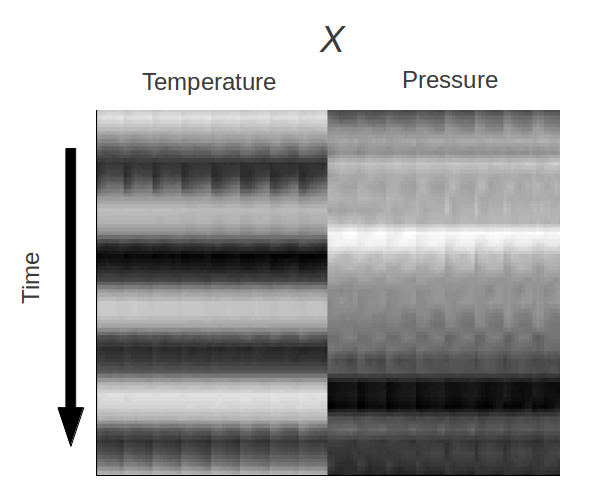
\includegraphics[width=1.0\textwidth]{./var_data_example.png}
	\caption{Input data comprised of temperature and pressure values on a small grid region}
\end{subfigure}
\\
\begin{subfigure}{0.2\textwidth}
	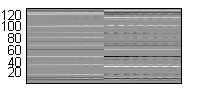
\includegraphics[width=1.0\textwidth]{./var_params_lag_1.png}
	\caption{Trained model coefficients assuming a lag order of 1}
\end{subfigure}
\begin{subfigure}{0.6\textwidth}
	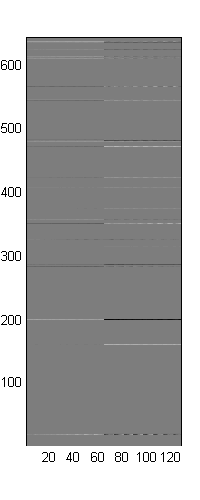
\includegraphics[width=1.0\textwidth]{./var_params_lag_5.png}
	\caption{Trained model coefficients assuming a lag order of 5}
\end{subfigure}
\caption{An illustrative example of the input data $\VARdata$ and trained output model $\VARmodel$ obtained using different lag parameters. This particular data is comprised of hourly samples over a 4-day window. Each row corresponds to all the observed values at a particular timestep, where the 2D gridded values for each variable type (in this case, surface temperature and pressure) are reshaped in into a row vector. Note that the large, monochrome gray regions in each $\VARmodel$ indicates significant sparsity of the model, which was not expected before using lasso regularization. }
\label{fig:var_data_example}
\end{figure}

TODO: Image showing heat-map evolution of temperature, pressure values, with 1 row per timestep and 1 column per variable. Indicate how grid of values is remapped to a single section of a row.

There are several possible reasons for this which we intend to investigate. First, the VAR model assumes a \emph{stationary} process, and our current preprocessing of the data before fitting the model may not guarantee this assumption. Additionally, there may be endogenous variables which affect the predictions which we are not yet including in the model (eg: wind speeds, elevation, etc.). 

Citation test: \cite{Durban2001}.

\bibliographystyle{unsrt}
\bibliography{10_701_Project_Refs}

\end{document}